%% Included in decks: slidemage-manual, slidemage-manual-copy
%%

% SlideMage manual, chapter "The big picture": templates. The two crops are
% the same slide (1wa) compiled under SlideMage's own template and under the
% stress-test template (tests/fixtures/template_stress/, a test template that
% changes every layout setting); see tools/manual/README.md. The color strip is
% live: it shows the palette of the template this deck uses.
\setSlideVersion{1-1-0}
\providecommand{\templatecrop}[2]{% image, caption
	\begin{tabular}[t]{@{}c@{}}
		{\setlength{\fboxsep}{0pt}\setlength{\fboxrule}{0.4pt}%
		\fcolorbox{c_primary_gray}{white}{#1}}\\[-1pt]
		{\scriptsize #2}
	\end{tabular}}
\begin{standardframe}{One look, several institutions}
	\small
	How a slide looks -- colors, logo, title bar, footer -- is set by a
	\emph{template}, not by the slide. A deck names its template once, so one slide
	appears in a different design in each deck -- below, one slide of this manual
	under two templates.
	\par\medskip
	\begin{columns}[T,onlytextwidth]
		\begin{column}{0.57\linewidth}
			\templatecrop{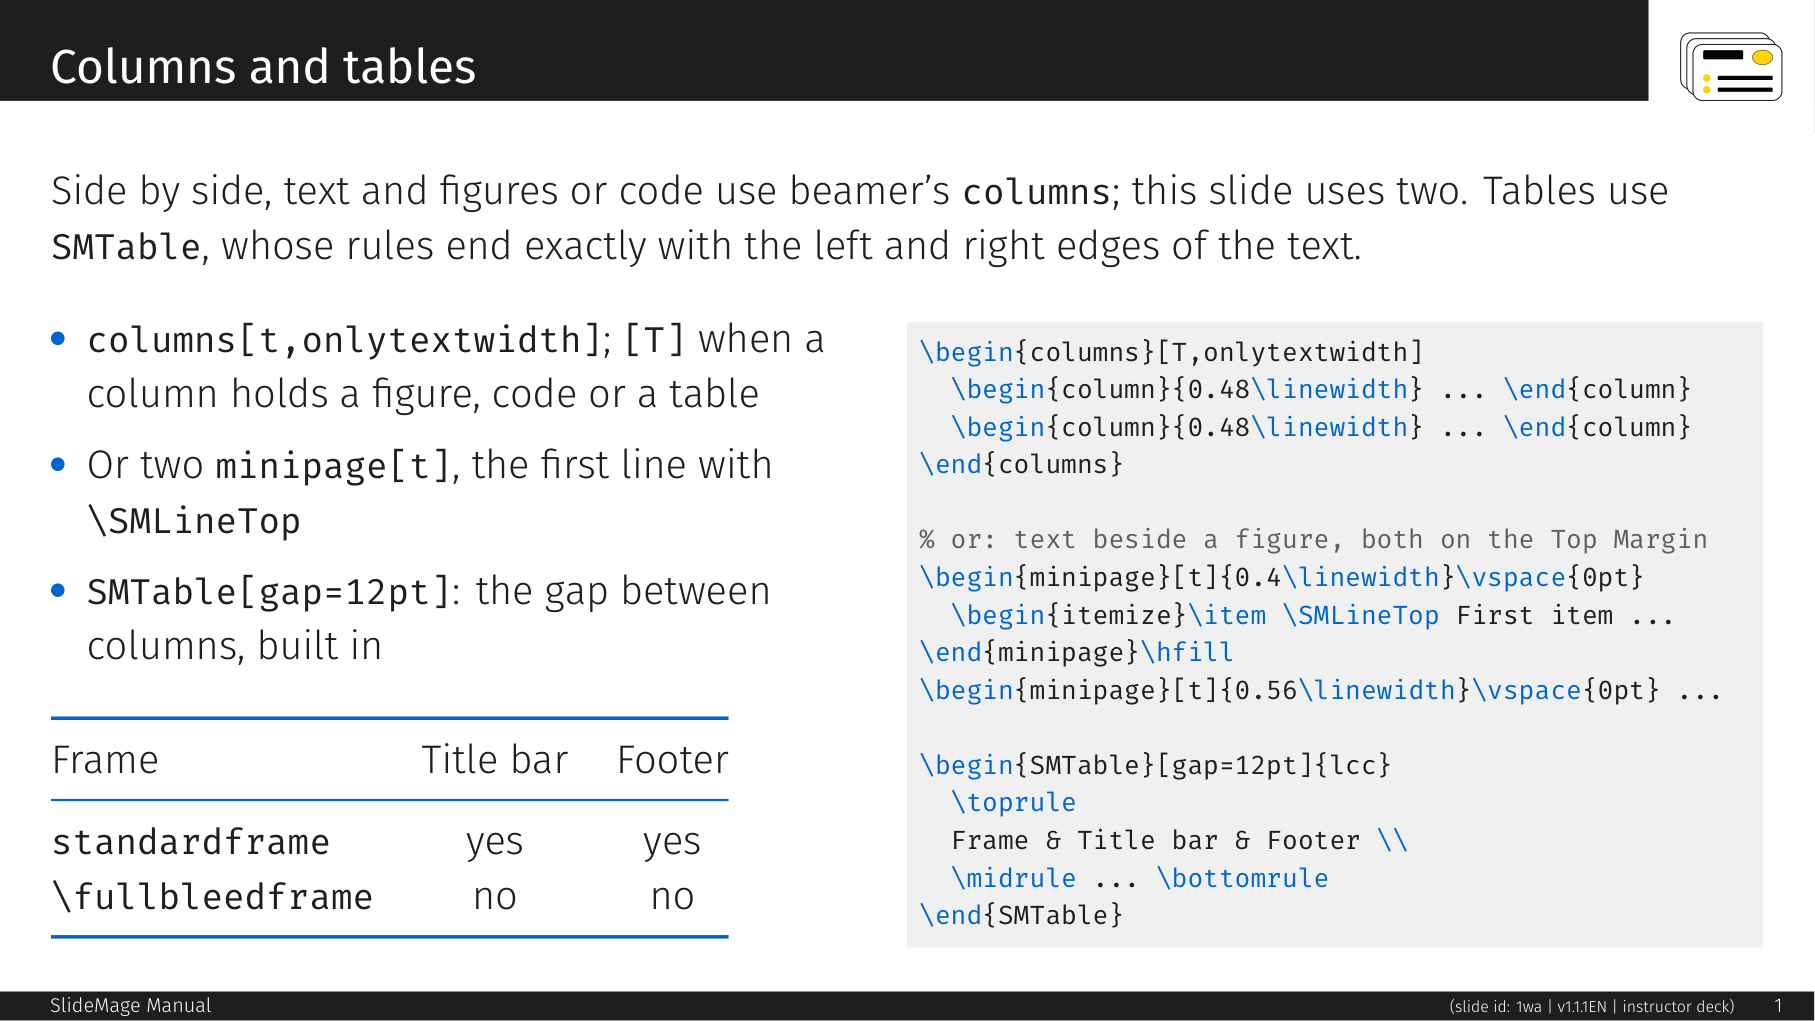
\includegraphics[width=98pt]{media/screenshot-slide-template-slidemage.png}}{SlideMage template} \hspace{4pt}
			\templatecrop{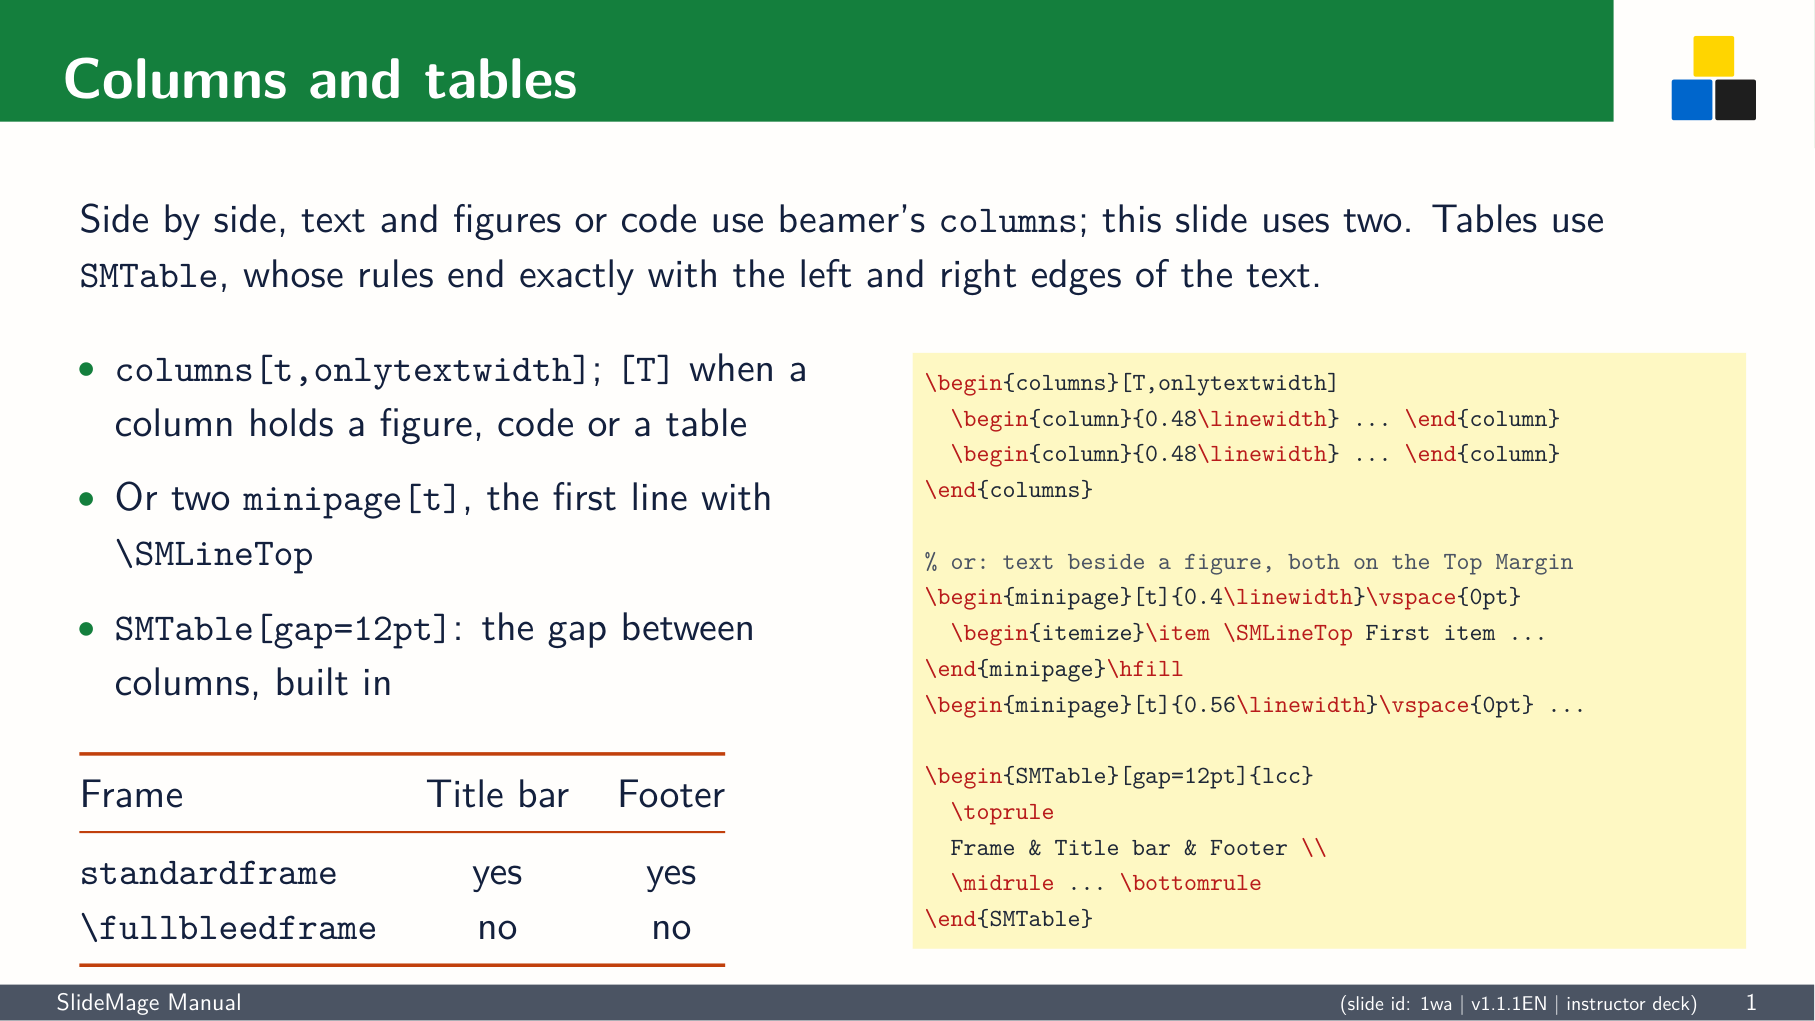
\includegraphics[width=98pt]{media/screenshot-slide-template-stress.png}}{Stress-test template}
		\end{column}
		\begin{column}{0.40\linewidth}
			\shrinklists{1}
			\begin{itemize}
				\item A template is one small file, \SMCode{Slidemaster\_preamble\_<name>.tex}
				\item SlideMage brings its own; for your institution, copy it and change colors and logo
			\end{itemize}
%			\smallskip
%			\begin{tikzpicture}[x=9.5pt, y=9.5pt]
%				\foreach \c [count=\i from 0] in {c_primary_dark, c_primary_highlight, c_primary_gray, c_primary_white, c_secondary_violet, c_tertiary_violet, c_secondary_blue, c_tertiary_blue, c_secondary_green, c_tertiary_green, c_secondary_red, c_tertiary_red, c_secondary_orange, c_tertiary_orange, c_secondary_yellow, c_tertiary_yellow, c_tertiary_gray, c_custom_gray, c_custom_red, c_custom_green, c_custom_brown}%
%					\fill[\c, draw=c_primary_gray, line width=0.2pt] ({mod(\i,11)},{-floor(\i/11)}) rectangle ++(0.85,0.85);
%			\end{tikzpicture}
		\end{column}
	\end{columns}
\end{standardframe}
